\section{Progettazione}
\label{sec:Progettazione}

\subsection{Uso di pattern}
\label{sec:UsoDiPattern}
L'utilizzo di un pattern influenza significativamente la progettazione di un sistema, o perlomeno di una sua parte. Abbiamo fatto uso del pattern Command, che ci ha suggerito le linee guida per la realizzazione del men�, che � composto da voci di men� che, se selezionate, fanno partire l'esecuzione di uno o pi� comandi.

L'utilizzo di questo pattern quindi ci ha portato a definire le classi Men�, MenuItem (le voci del men�) e Command.
I comandi sono realizzati come classi che hanno la responsabilit� dell'esecuzione del comando che implementano. 
Il men� viene istanziato in forme diverse a seconda del tipo di utente che accede al sistema, abilitando o meno alcune operazioni.

\subsection{Descrizione del sistema e interazioni fra le classi}
\label{sec:DescrizioneDelSistemaEInterazioniFraLeClassi}
La classe \textbf{Sistema} ha un ruolo fondamentale nell'applicazione, in quanto crea gli oggetti che sono alla base del suo funzionamento.
In particolare, questi oggetti sono:
\begin{itemize}
 \item Forum
 \item ListaUtentiForum
 \item Disegnatore
 \item Menu
\end{itemize}

Inoltre il sistema dopo aver autorizzato un utente registrato a utilizzare il forum, delega agli oggetti che ha creato il recupero delle informazioni memorizzate in precedenza sui file.

Il \textbf{Forum} contiene i riferimenti ai gruppi di discussione e fornisce agli oggetti di classe Command l'accesso ai messaggi memorizzati. Tutta la gestione dei gruppi di discussione passa attraverso questa classe.

Un \textbf{GruppoDiscussione} � formato da un insieme di messaggi, strutturato come una sequenza di domande seguite da eventuali risposte. Le domande e le risposte sono tutte istanze della classe \textbf{Messaggio}. E' compito di GruppoDiscussione mantenere su file i messaggi in modo ordinato.

\textbf{ListaUtentiForum} ha i riferimenti agli utenti registrati nel sistema e dunque ha accesso a tutti i loro dati, permettendo il loro utilizzo alle classi che ne fanno richiesta. Questa classe si preoccupa anche di garantire la persistenza dei dati di cui � responsabile.

L'utente semplice � rappresentato dalla classe \textbf{Utente}. Da questa ereditano le classi \textbf{Tutor} e \textbf{Amministratore}, che hanno in pi� dei riferimenti a un insieme di gruppi per i quali hanno diritto a rispondere.
Le operazioni di responsabilit� dell'amministratore vengono rese disponibili dal Menu che viene a lui istanziato.

Alla classe \textbf{Disegnatore} vengono indirizzate le richieste di visualizzazione dell'output in modo da dare un aspetto omogeneo all'interfaccia utente.

La classe \textbf{Menu} possiede i riferimenti ai MenuItem, ovvero le voci di menu che possono presentarsi agli utenti. I MenuItem vengono istanziati dal costruttore di questa classe a seconda dell'utente che sta utilizzando il sistema. I \textbf{MenuItem} a loro volta hanno i riferimenti a un insieme di \textbf{Command} che implementano i comandi associati alle voci di menu disponibili. Selezionare un MenuItem equivale quindi a eseguire in maniera ordinata le Command a cui fa riferimento. Tutti i comandi sono implementati nel metodo \emph{execute()} di classi derivate da Command. Queste ultime, per eseguire i propri compiti, dispongono dei riferimenti alle classi principali del sistema (Forum, ListaUtentiForum, Disegnatore).

\subsection{Diagramma UML}
\label{sec:DiagrammaUML}
Il diagramma UML risultante dalla progettazione e dalle sue successive revisioni � il seguente:
\begin{figure}[!ht]
      \centering
      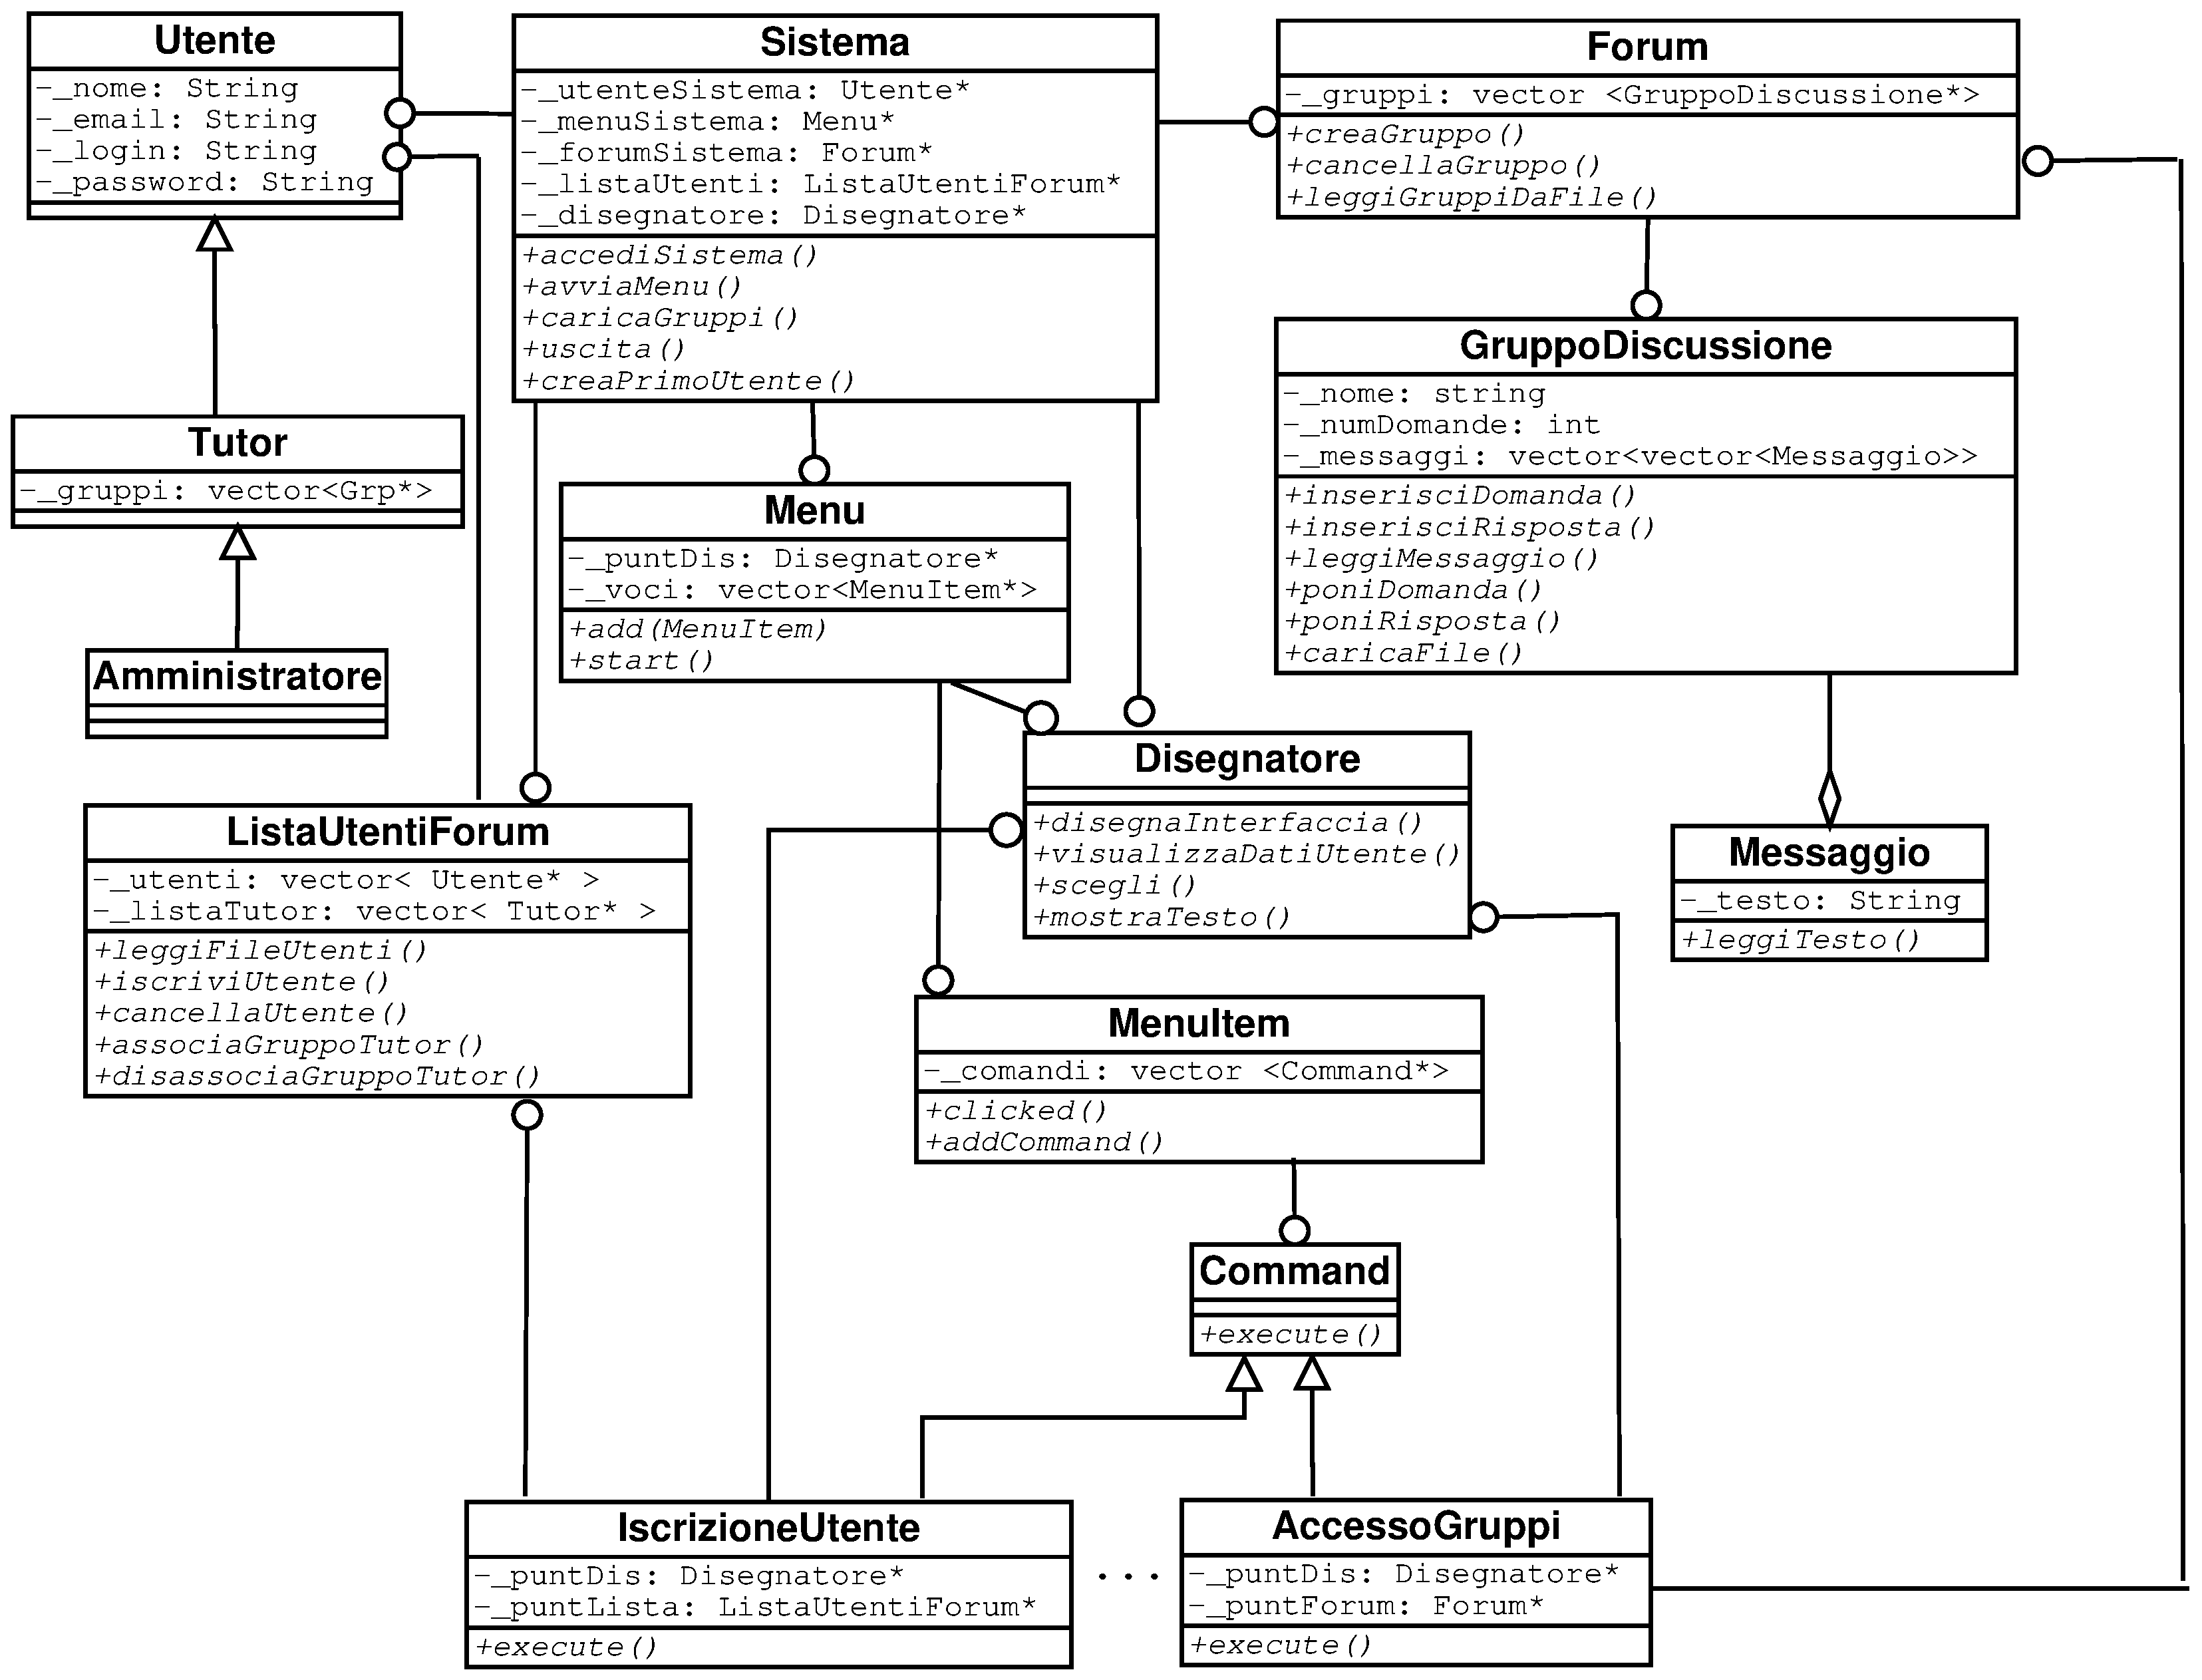
\includegraphics[angle = 90, width=\textwidth, height = \textheight]{UML.eps}
      %\caption{Diagramma delle classi}
\end{figure}

